\section{Akustik}

\subsection{Teminologie}

\paragraph{Ton}

Eine harmonische Schallwelle wird als \textbf{Ton} bezeichnet.

Ein (reiner) Ton entspricht also einer \textbf{Schallschwingung}, die \textbf{eine einzige Frequenz} enthält.

\medskip
\paragraph{Klang}

Eine \textbf{Überlagerung} von harmonischen Schwingungen, deren \textbf{Frequenzen} in einem 
\textbf{ganzzahligen Verhältnis} zur tiefsten Frequenz, zur Frequenz des \textbf{Grundtons}, stehen, wird \textbf{Klang} genannt. 

\medskip
\paragraph{Geräusch}

Bei einem \textbf{Geräusch} besteht das Frequenzspektrum nicht mehr aus einzelnen diskreten Linien, sondern weist in einem bestimmten Frequenzbereich eine  \textbf{kontinuierliche Verteilung} auf.


\subsection{Pegel}

\begin{minipage}[t]{0.48\columnwidth}
    \paragraph{'Einheit': Bel}

    $$ \boxed{ \text{Pegel} = \log \left( \frac{x}{b_0} \right) } $$
    $$ \boxed{ x = b_0 \cdot 10^{\text{Pegel} } } $$ 
\end{minipage}
\hfill
\begin{minipage}[t]{0.48\columnwidth}
    \paragraph{'Einheit': Dezibel}

    $$ \boxed{ \text{Pegel} = 10 \cdot \log \left( \frac{x}{b_0} \right) } $$ 
    $$ \boxed{ x = b_0 \cdot 10^{\left( \frac{\text{Pegel}}{10} \right) } } $$
\end{minipage}

\renewcommand{\arraystretch}{1.3}
\begin{ctabular}{clc}
    Pegel   & Dimensionslose Grösse     & $[\text{Pegel}] =  1$ \\
    $x$     & Zu vergleichende Grösse   & $[x]$                 \\
    $b_0$   & Basisgrösse               & $[b_0] = [x]$
\end{ctabular}
\renewcommand{\arraystretch}{1}


\subsection{Schallintensität}

\begin{minipage}{0.48\columnwidth}
    $$ \boxed{ L_I = 10 \cdot \log \left( \frac{I}{I_0} \right) } $$ 
\end{minipage}
\hfill
\begin{minipage}{0.48\columnwidth}
    $$ \boxed{ L_p = 20 \cdot \log \left( \frac{p_{\rm eff}}{p_{\rm eff0}} \right) } $$ 
\end{minipage}

$$ \boxed{ p_{\rm eff} = \frac{\Delta p_0}{\sqrt{2}} } $$

\renewcommand{\arraystretch}{1.3}
\begin{ctabular}{clc}
    $L_I$           & Schallintensitätspegel        & $[L_I] = \deci\bel$                   \\
    $L_p$           & Schalldruckpegel              & $[L_p] = \deci\bel$                   \\
    $I$             & Intensität                    & $[I] = \frac{\watt}{\meter\squared}$  \\
    $p_{\rm eff}$   & Schalldruck (Effektivwert)    & $[p_{\rm eff}] = \pascal$             \\
    $\Delta p_0$    & Druckamplitude                & $[\Delta p_0] = \pascal$ 
\end{ctabular}

\begin{ctabular}{cll}
    $I_0$           & Bezugsintensität  & $I_0 = 10^{-12} \, \frac{\watt}{\meter\squared}$ \\
    $p_{\rm eff0}$  & Bezugsschalldruck & $p_{\rm eff0} = 2 \cdot 10^{-5} \pascal$
\end{ctabular}
\renewcommand{\arraystretch}{1}



\subsection{Intensität bei Kugelwellen}

\vspace{-0.4cm}

\renewcommand{\arraystretch}{3}
\begin{tabular}{@{}lll@{}}
					 & \textbf{ohne Dämpfung}                                               & \textbf{mit Dämpfung} \\
	Energieerhaltung & $\boxed{ I(r) = \frac{P}{4 \, \pi \, r^2} }$                         & $\boxed{ I(r) = \frac{P}{4 \, \pi \, r^2} \, \e^{- \alpha r}}$                       \\ 

	Verhältnis 		 & $\boxed{ \frac{I_2}{I_1} = \frac{r_1^2}{r_2^2} }$                    & $\boxed{ \frac{I_2}{I_1} = \frac{r_1^2}{r_2^2} \, \e^{- \alpha (r_2 - r_1)} }$        \\

	Pegel 			 & $\boxed{ L_2 = L_1 - 20 \cdot \log \left( \frac{r_2}{r_1} \right)}$  & $\boxed{ L_2 = L_1 - 20 \cdot \log \left( \frac{r_2}{r_1} \right) - K (r_2 - r_1)  }$ \\
\end{tabular}



\renewcommand{\arraystretch}{1.2}
\begin{ctabular}{clc}
	$I(r)$      & Intensität                                                            & $[I(r)] = \frac{\watt}{\meter\squared}$   \\
	$P$         & Leistung                                                              & $[P] = \watt$                             \\
	$r_i$       & Abstand (Radius) zum Wellenursprung                                   & $[r_i] = \meter\squared$                  \\
	$L_i$       & Pegel                                                                 & $[L_i] = \deci\bel$                       \\
	$\alpha$    & Absorptionsgrad ($\alpha = 1-R$, siehe \ref{Reflexion} )              & $[\alpha] = 1$                            \\
	$K$         & Dämpfung                                                              & $[K] = \frac{\deci\bel}{\meter}$
\end{ctabular}
\renewcommand{\arraystretch}{1}



\subsection{Verschiedene Schallquellen}

\begin{center}
    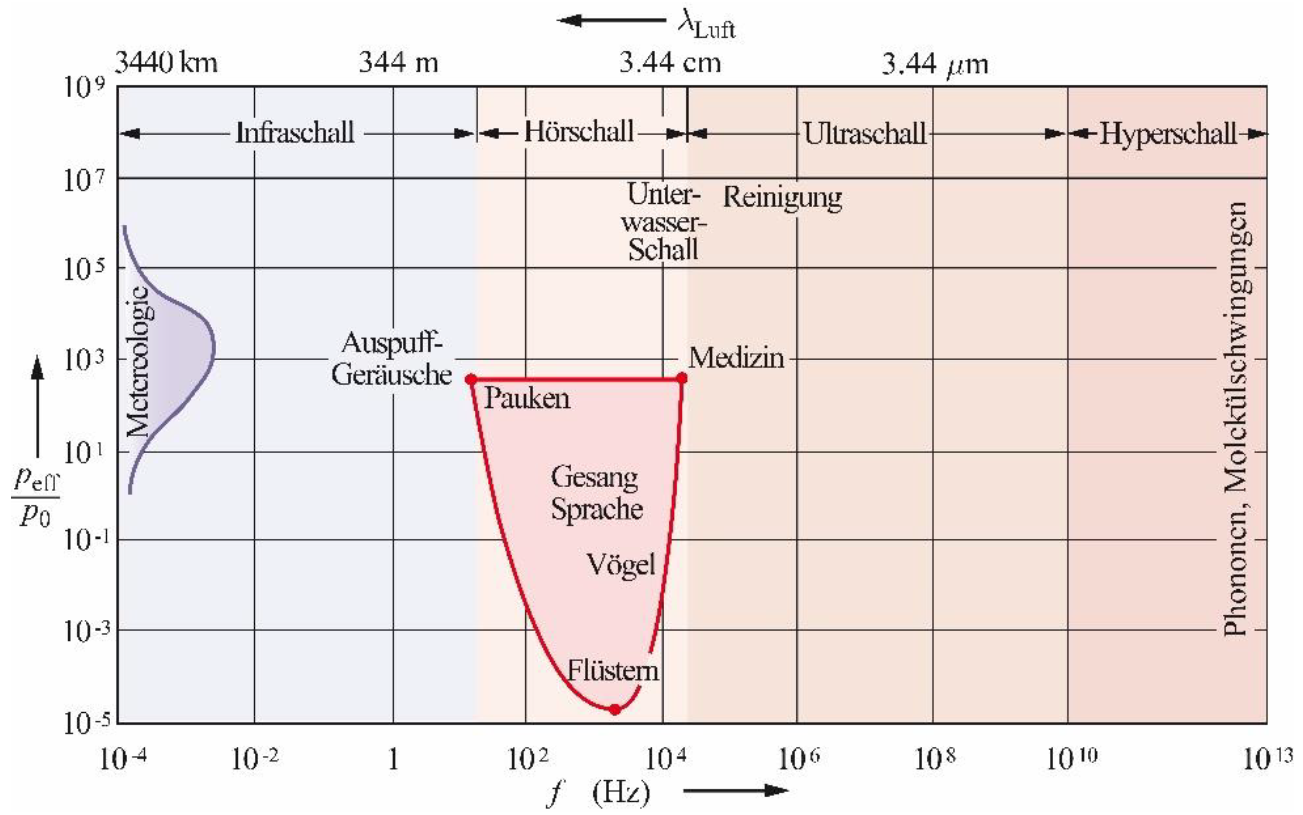
\includegraphics[width=0.9\columnwidth]{images/schallquellen.png}
\end{center}


\subsection{PHON-Skala}

\begin{center}
    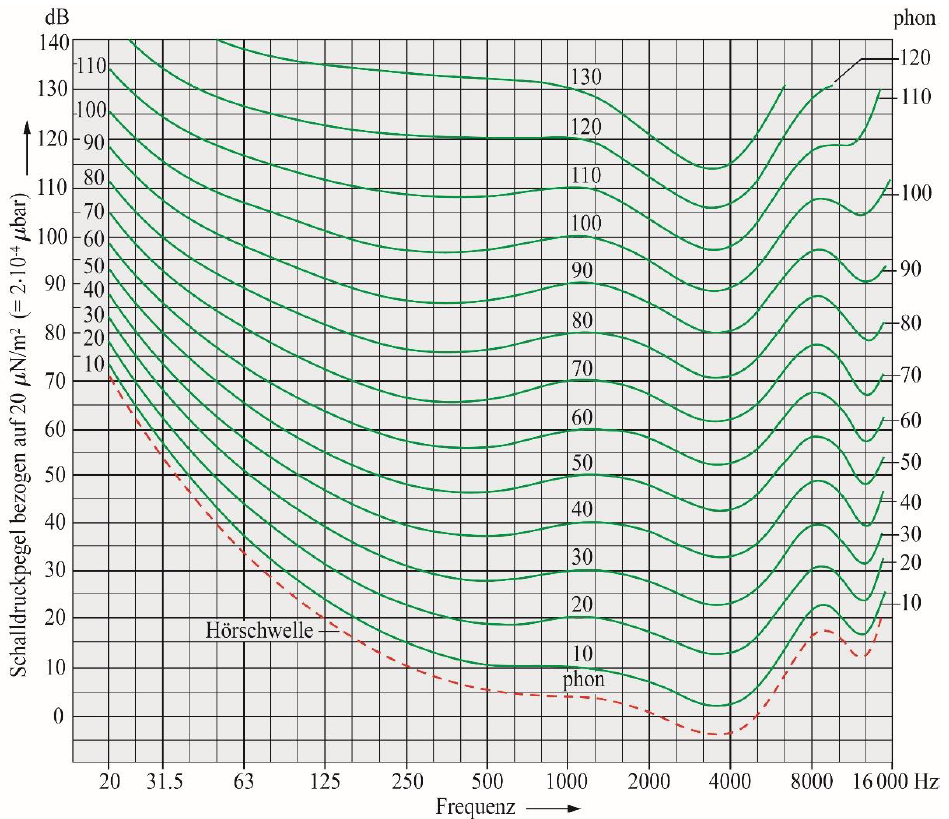
\includegraphics[width=\columnwidth]{images/phon_skala.png}
\end{center}



\subsection{Schalldämpfung / Schalldämmung}

\subsubsection{Schalldämpfung}

Schalldämpfung bedeutet eine \textbf{Abschwächung} der Schallwellen durch \textbf{Absorption}. 

Schallenergie wird in \textbf{'Wärme' umgewandelt}, d.h. durch die Absorption von Energie werden das von den Schallwellen
durchdrungene Medium oder die das Schallfeld begrenzenden Körper \textbf{erwärmt}.

\medskip
\paragraph{Verschiedene Arten von Absorption für Schalldämpfung Innen}

\begin{itemize}
	\item Poröse Schicht (mit oder ohne perforierte Abdeckung) 
	\item Akustikplatte 
	\item Plattenresonator
	\item Helmholtz-Resonator
\end{itemize}


\subsubsection{Schalldämmung} 

Schalldämmung ist die \textbf{Behinderung der Schallausbreitung} durch \textbf{reflektierende} Hindernisse. 
Mauern, Türen und Fenster bewirken eine Schalldämmung für den von aussen in das Gebäude eindringenden Schall. 
Auch die Ausbreitung von Schall innerhalb eines Gebäudes wird durch die Schalldämmung von Zwischenwänden und Türen abgeschwächt. 
Im Freien wird durch Schallschutzwände eine Schalldämmung für die dahinterliegenden Gebäude erreicht.


\subsection{Schalldämmung / Schalldämm-Mass}

Bei der Schallübertragung muss zwischen \textbf{Luftschall} und \textbf{Körperschall} unterschieden werden.


\subsubsection{Luftschalldämmung}

Es gibt Schallquellen, die ihre Schallenergie (fast) ausschliesslich in die Luft abstrahlen.

Beispiele: menschliche Stimme, Geigen, Lautsprecher und Blasinstrumente


\subsubsection{Körperschalldämmung}

Andere Schallerzeuger übertragen die Schallschwingungen nicht nur auf die Luft, sondern auch direkt auf feste Körper. 
Streichinstrumente, wie Cello oder Bassgeige, und Klavier oder Flügel übertragen die Schallschwingungen auch direkt auf den Fussboden. 
Wird ein Nagel in die Wand geschlagen, so wird ein grosser Anteil des erzeugten Schalls als Körperschall übertragen.

Beispiele: Trittschall, Wasserleitungsgeräusche


\subsection{Schalldämm-Mass}

$$ \boxed{ \mathcal{R} = 10 \cdot \left( \frac{P_1}{P_2} \right)  } $$


\subsection{Anhall / Nachhall}

\subsubsection{Anhall}

Es dauert eine gewisse Zeit, bis sich eine \text{konstante Energiedichte} der Schallwellen \text{im Raum aufgebaut} hat. Dieser Vorgang wird Anhall genannt. Wegen der logarithmischen Empfindlichkeit des Ohrs \text{wird er praktisch nicht wahrgenommen}.


\subsubsection{Nachhall}

Die von den Begrenzungsflächen des Raumes mehrfach reflektierten Wellen bewirken andererseits, dass beim \text{plötzlichen Abschalten} einer Schallquelle der Schall nicht sofort verschwindet, sondern \text{allmählich abklingt}. Dieses Phänomen wird Nachhall genannt und ist im Gegensatz zum Anhall \text{deutlich wahrnehmbar}.

\medskip
\textbf{Per Definition ist die Nachhallzeit jene Zeitspanne, in welcher der Schallpegel im Raum um 60 dB sinkt.}


\subsubsection{Nachhallzeit $\bm{T_N}$}

$$ \boxed{ T_N = 0.16 \, \frac{\second}{\meter} \frac{V}{\sum\limits_i \alpha_i A_i } } $$

\renewcommand{\arraystretch}{1.3}
\begin{ctabular}{clc}
    $T_N$       & Nachhallzeit & $[T_N] = \second$ \\
    $V$         & Raumvolumen & $[V] = \meter\cubed$ \\
    $\alpha_i$  & Absoptionsgrad & $[\alpha_i] = 1$ \\
    $A_i$       & Teilfläche der Raumbegrenzung mit Absorption $\alpha_i$ & $[A_i] = \meter\squared$ \\ 
\end{ctabular}
\renewcommand{\arraystretch}{1}

